\documentclass[12pt]{article}

\usepackage[utf8]{inputenc}
\usepackage[spanish]{babel}
\usepackage{amssymb, amsmath, geometry, graphicx, subcaption}

\setlength{\parindent}{0cm}
\geometry{letterpaper, margin=2.54cm}
\decimalpoint
\pagestyle{plain}

\title{
	Geometría Analítica Vectorial y Funciones Vectoriales \\
	\vspace{0.4cm}
	\Large Coordenadas Polares
}
\date{21 de junio de 2026}
\author{Rosendo Camal}

\begin{document}

% Portada
\maketitle

% Actividad 1
\section*{Actividad 1}
\textbf{Instrucciones:} Convertir a coordenadas cartesianas: $(8, 45^\circ)$.
\newline

\textbf{Respuesta:}

\begin{align*}
	(8, 45^\circ) &\Longrightarrow \left(r\cos\theta, r\sen\theta\right) \\
	\left(r, \theta\right) &\Longrightarrow \left(r\cos\theta, r\sen\theta\right) \\
	r &= 8 \\
	\theta &= 45^\circ \\
	(8, 45^\circ) &\Longrightarrow (8\cos45^\circ, 8\sen45^\circ)
\end{align*}

\begin{figure}[htb]
	\centering
	\begin{subfigure}[b]{0.40\linewidth}
		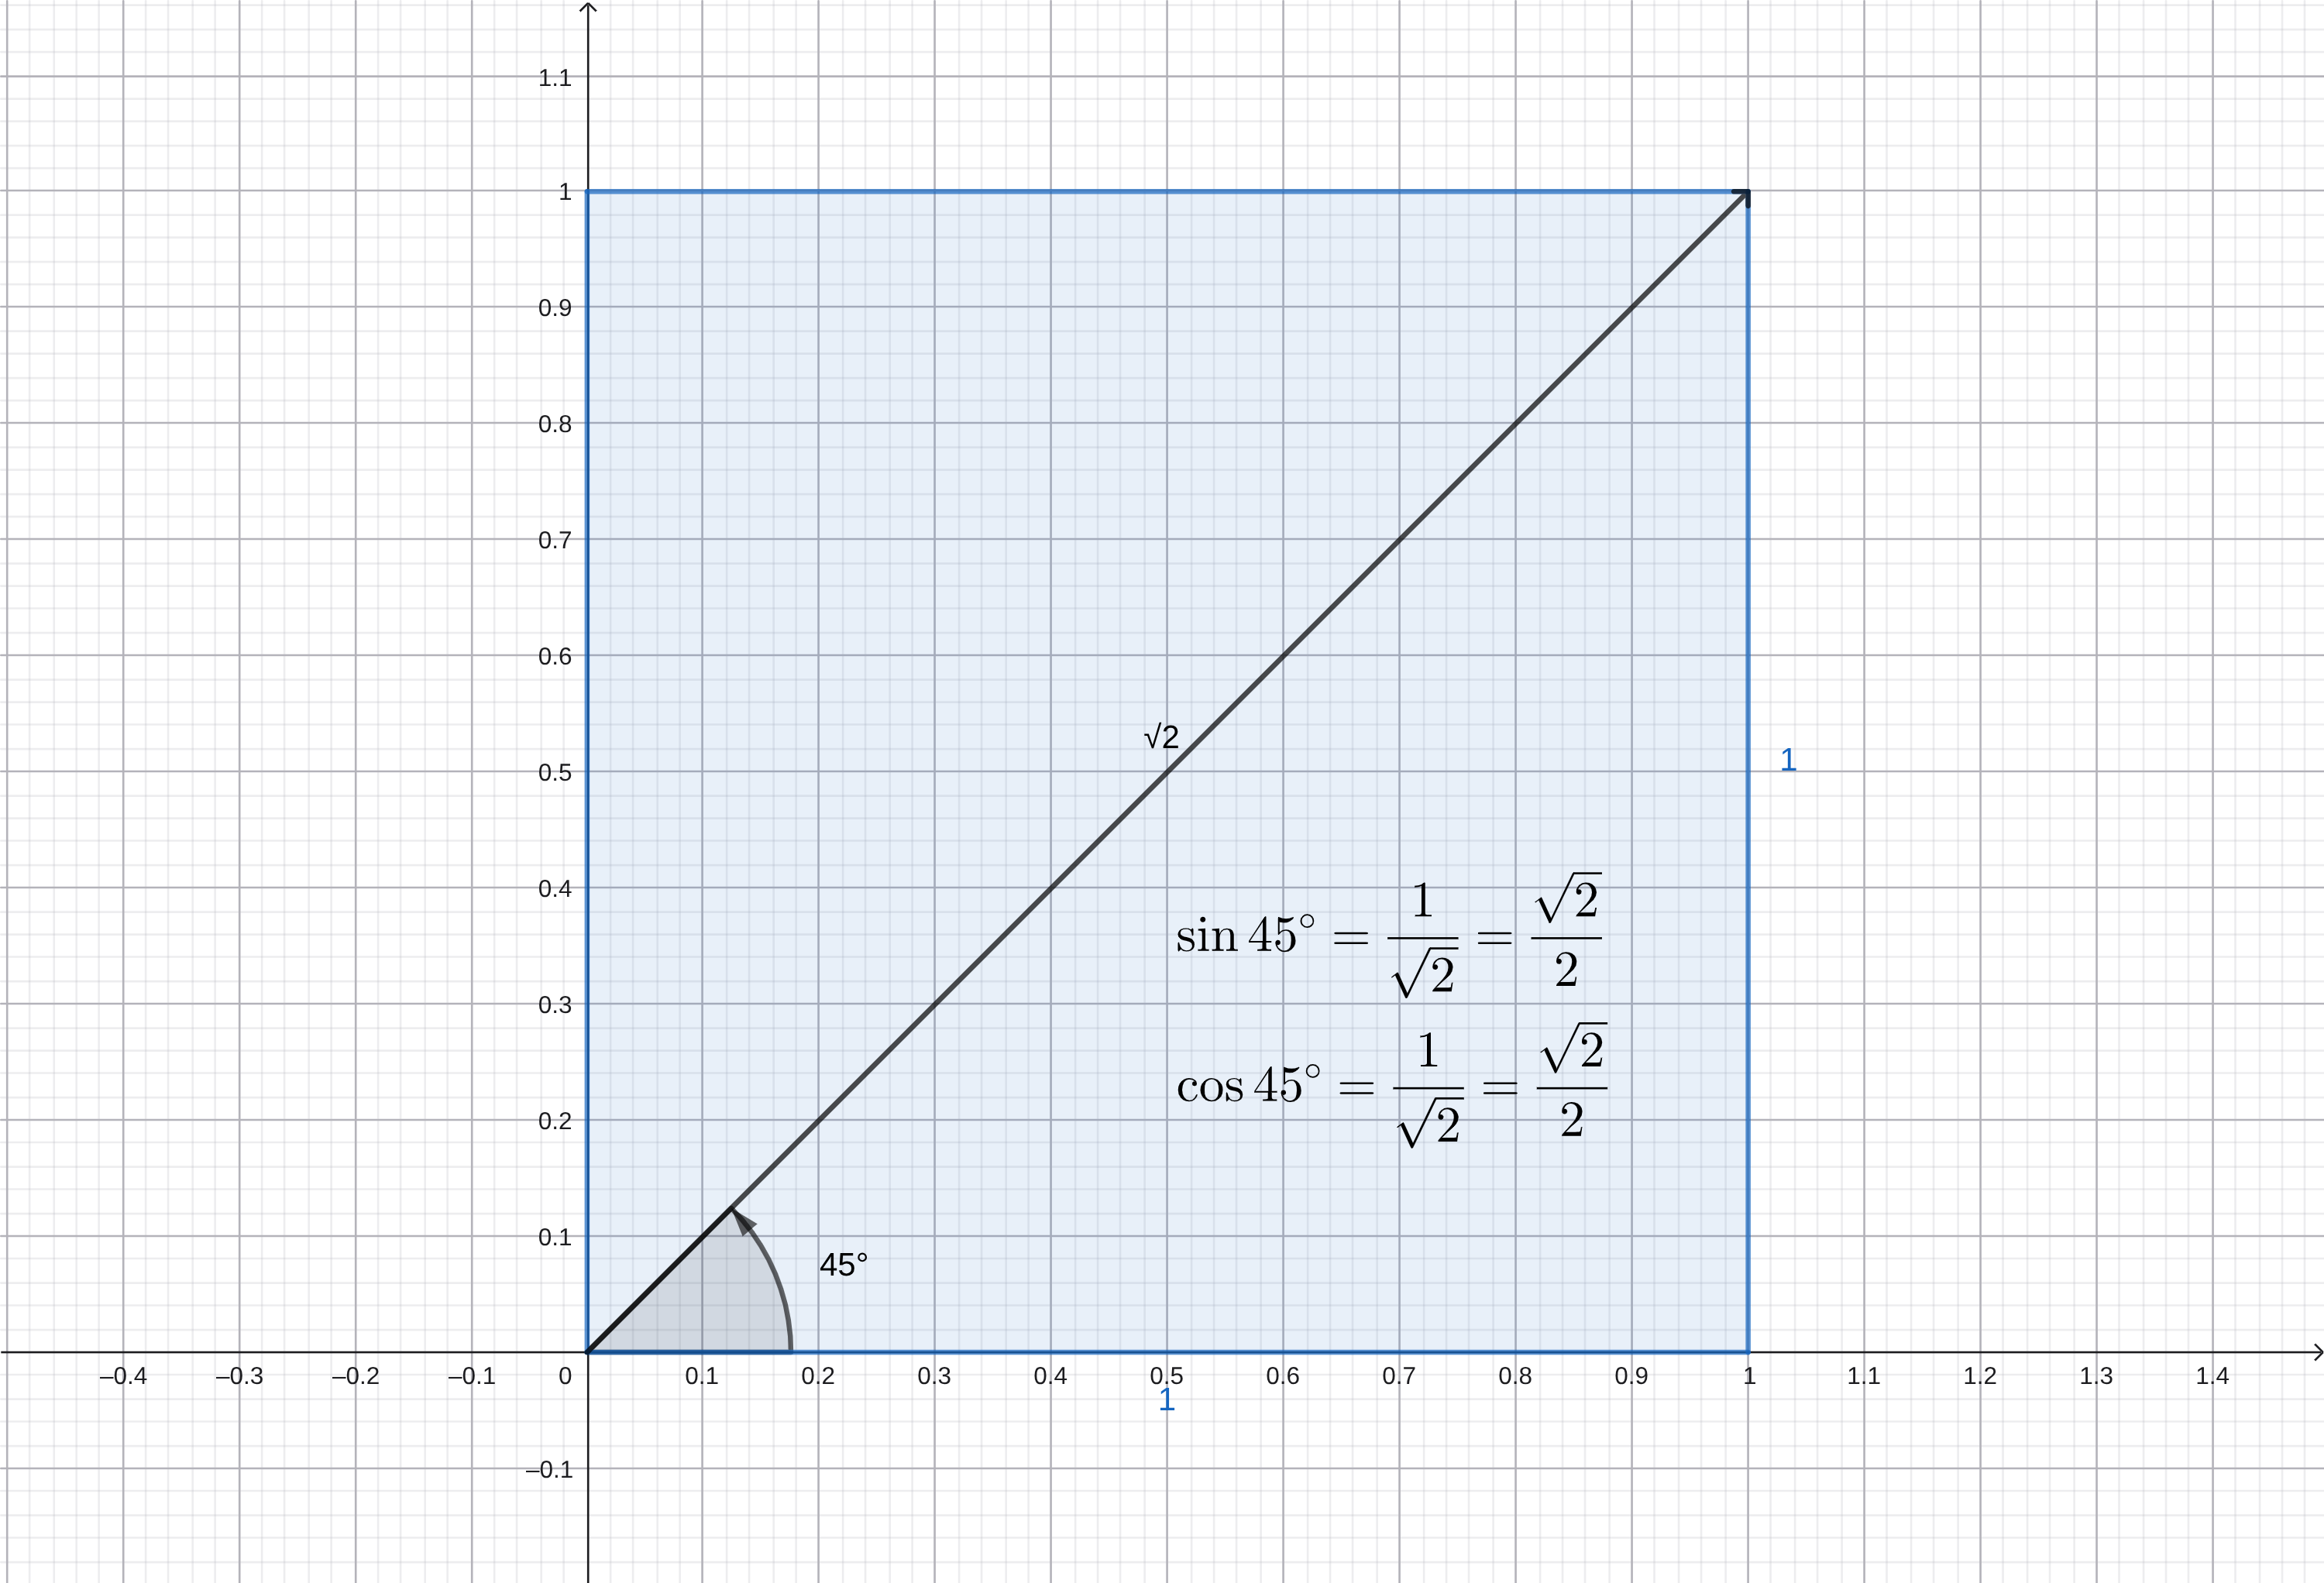
\includegraphics[width=\linewidth]{./geogebra-export1.png}
		\caption{$\sin$ y $\cos$ de $45^\circ$}
	\end{subfigure}
	\begin{subfigure}[b]{0.40\linewidth}
		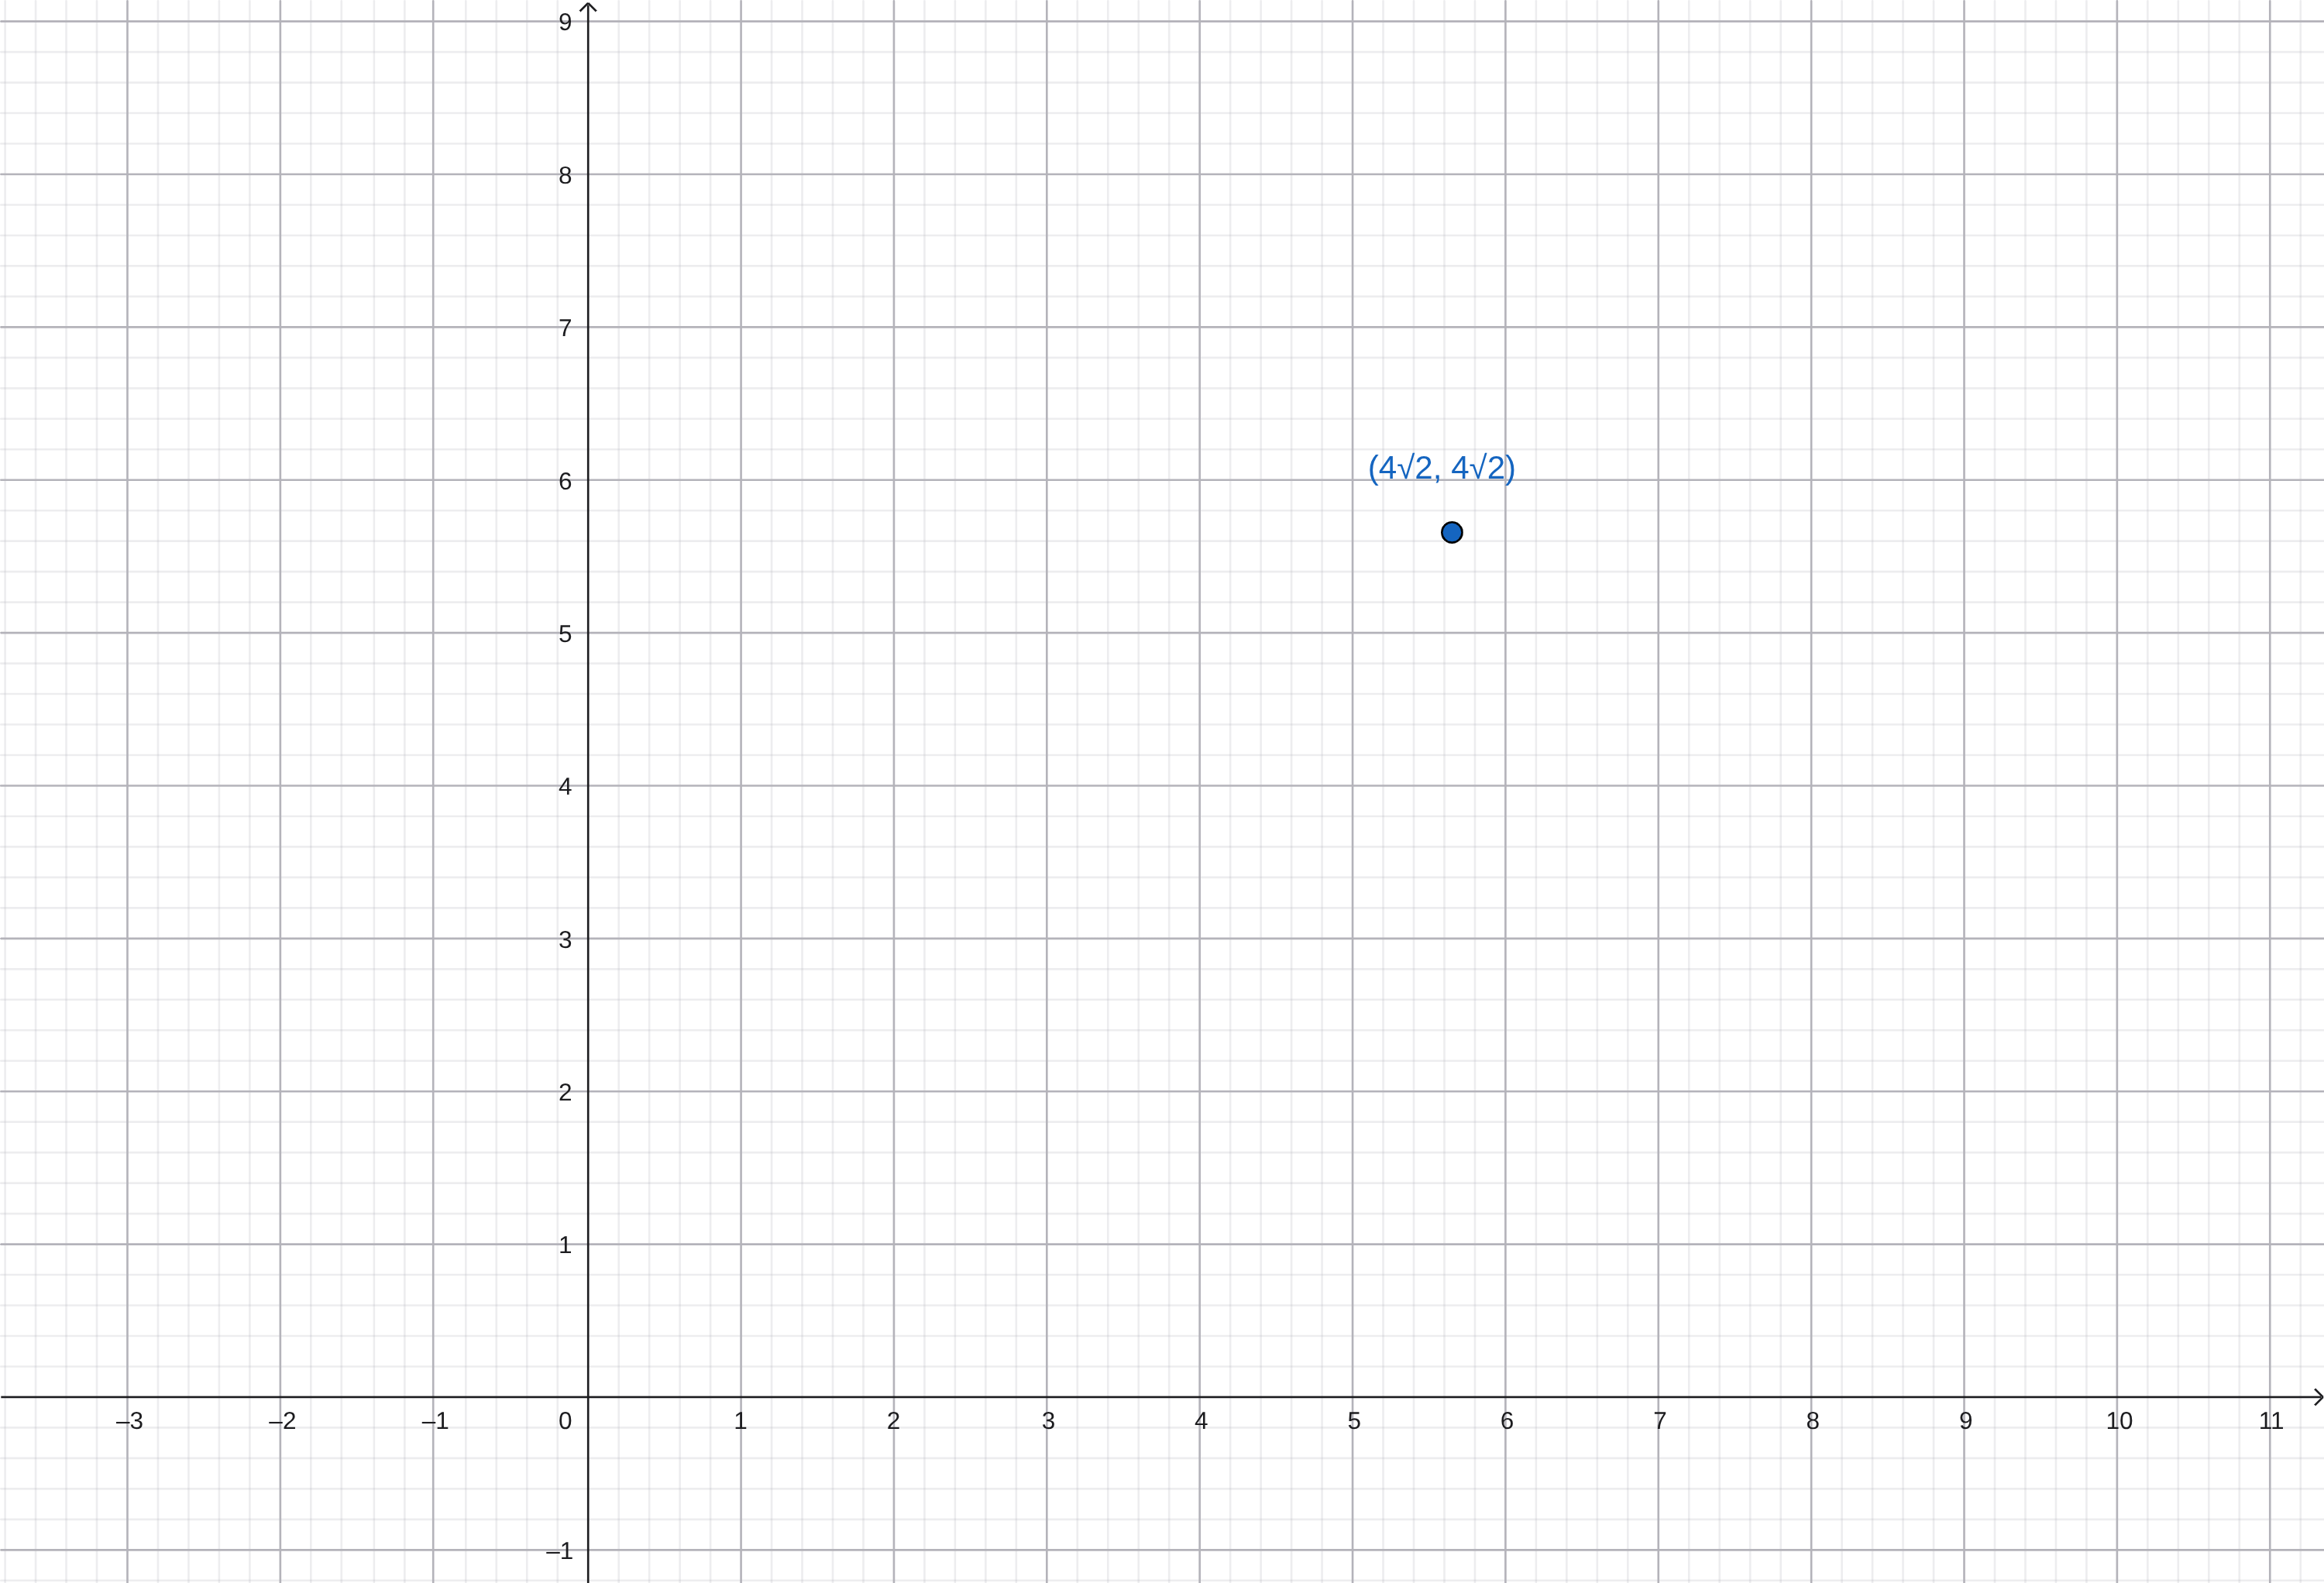
\includegraphics[width=\linewidth]{./geogebra-export3.png}
		\caption{Ubicación de $(4\sqrt{2}, 4\sqrt{2})$}
	\end{subfigure}
\end{figure}

\begin{align*}
	\left(8\cos45^\circ, 8\sen45^\circ\right) &\Longrightarrow \left(8\left(\frac{\sqrt{2}}{2}\right),  8\left(\frac{\sqrt{2}}{2}\right)\right) \\
	& \Longrightarrow \left(4\sqrt{2}, 4\sqrt{2}\right)
\end{align*}

% Actividad 2
\section*{Actividad 2}
\textbf{Instrucciones:} Convertir a coordenadas polares: $(6, 8)$.
\newline

\textbf{Respuesta:}

\begin{align*}
	(6, 8) = (x, y) &\Longrightarrow (r, \theta) \\
	&\Longrightarrow \left(\sqrt{x^2 + y^2}, \arctan\left(\frac{y}{x}\right)\right) \\
	&\Longrightarrow \left(\sqrt{6^2 + 8^2}, \arctan\left(\frac{8}{6}\right) \right) \\
	&\Longrightarrow \left(\sqrt{36 + 64}, \arctan\left(\frac{4}{3}\right)\right) \\
	&\Longrightarrow \left(\sqrt{100}, \tan^{-1}\left(\frac{4}{3}\right)\right) \\
	&\Longrightarrow \left(10, 53.13^\circ\right)
\end{align*}

\begin{figure}[htb]
	\centering
	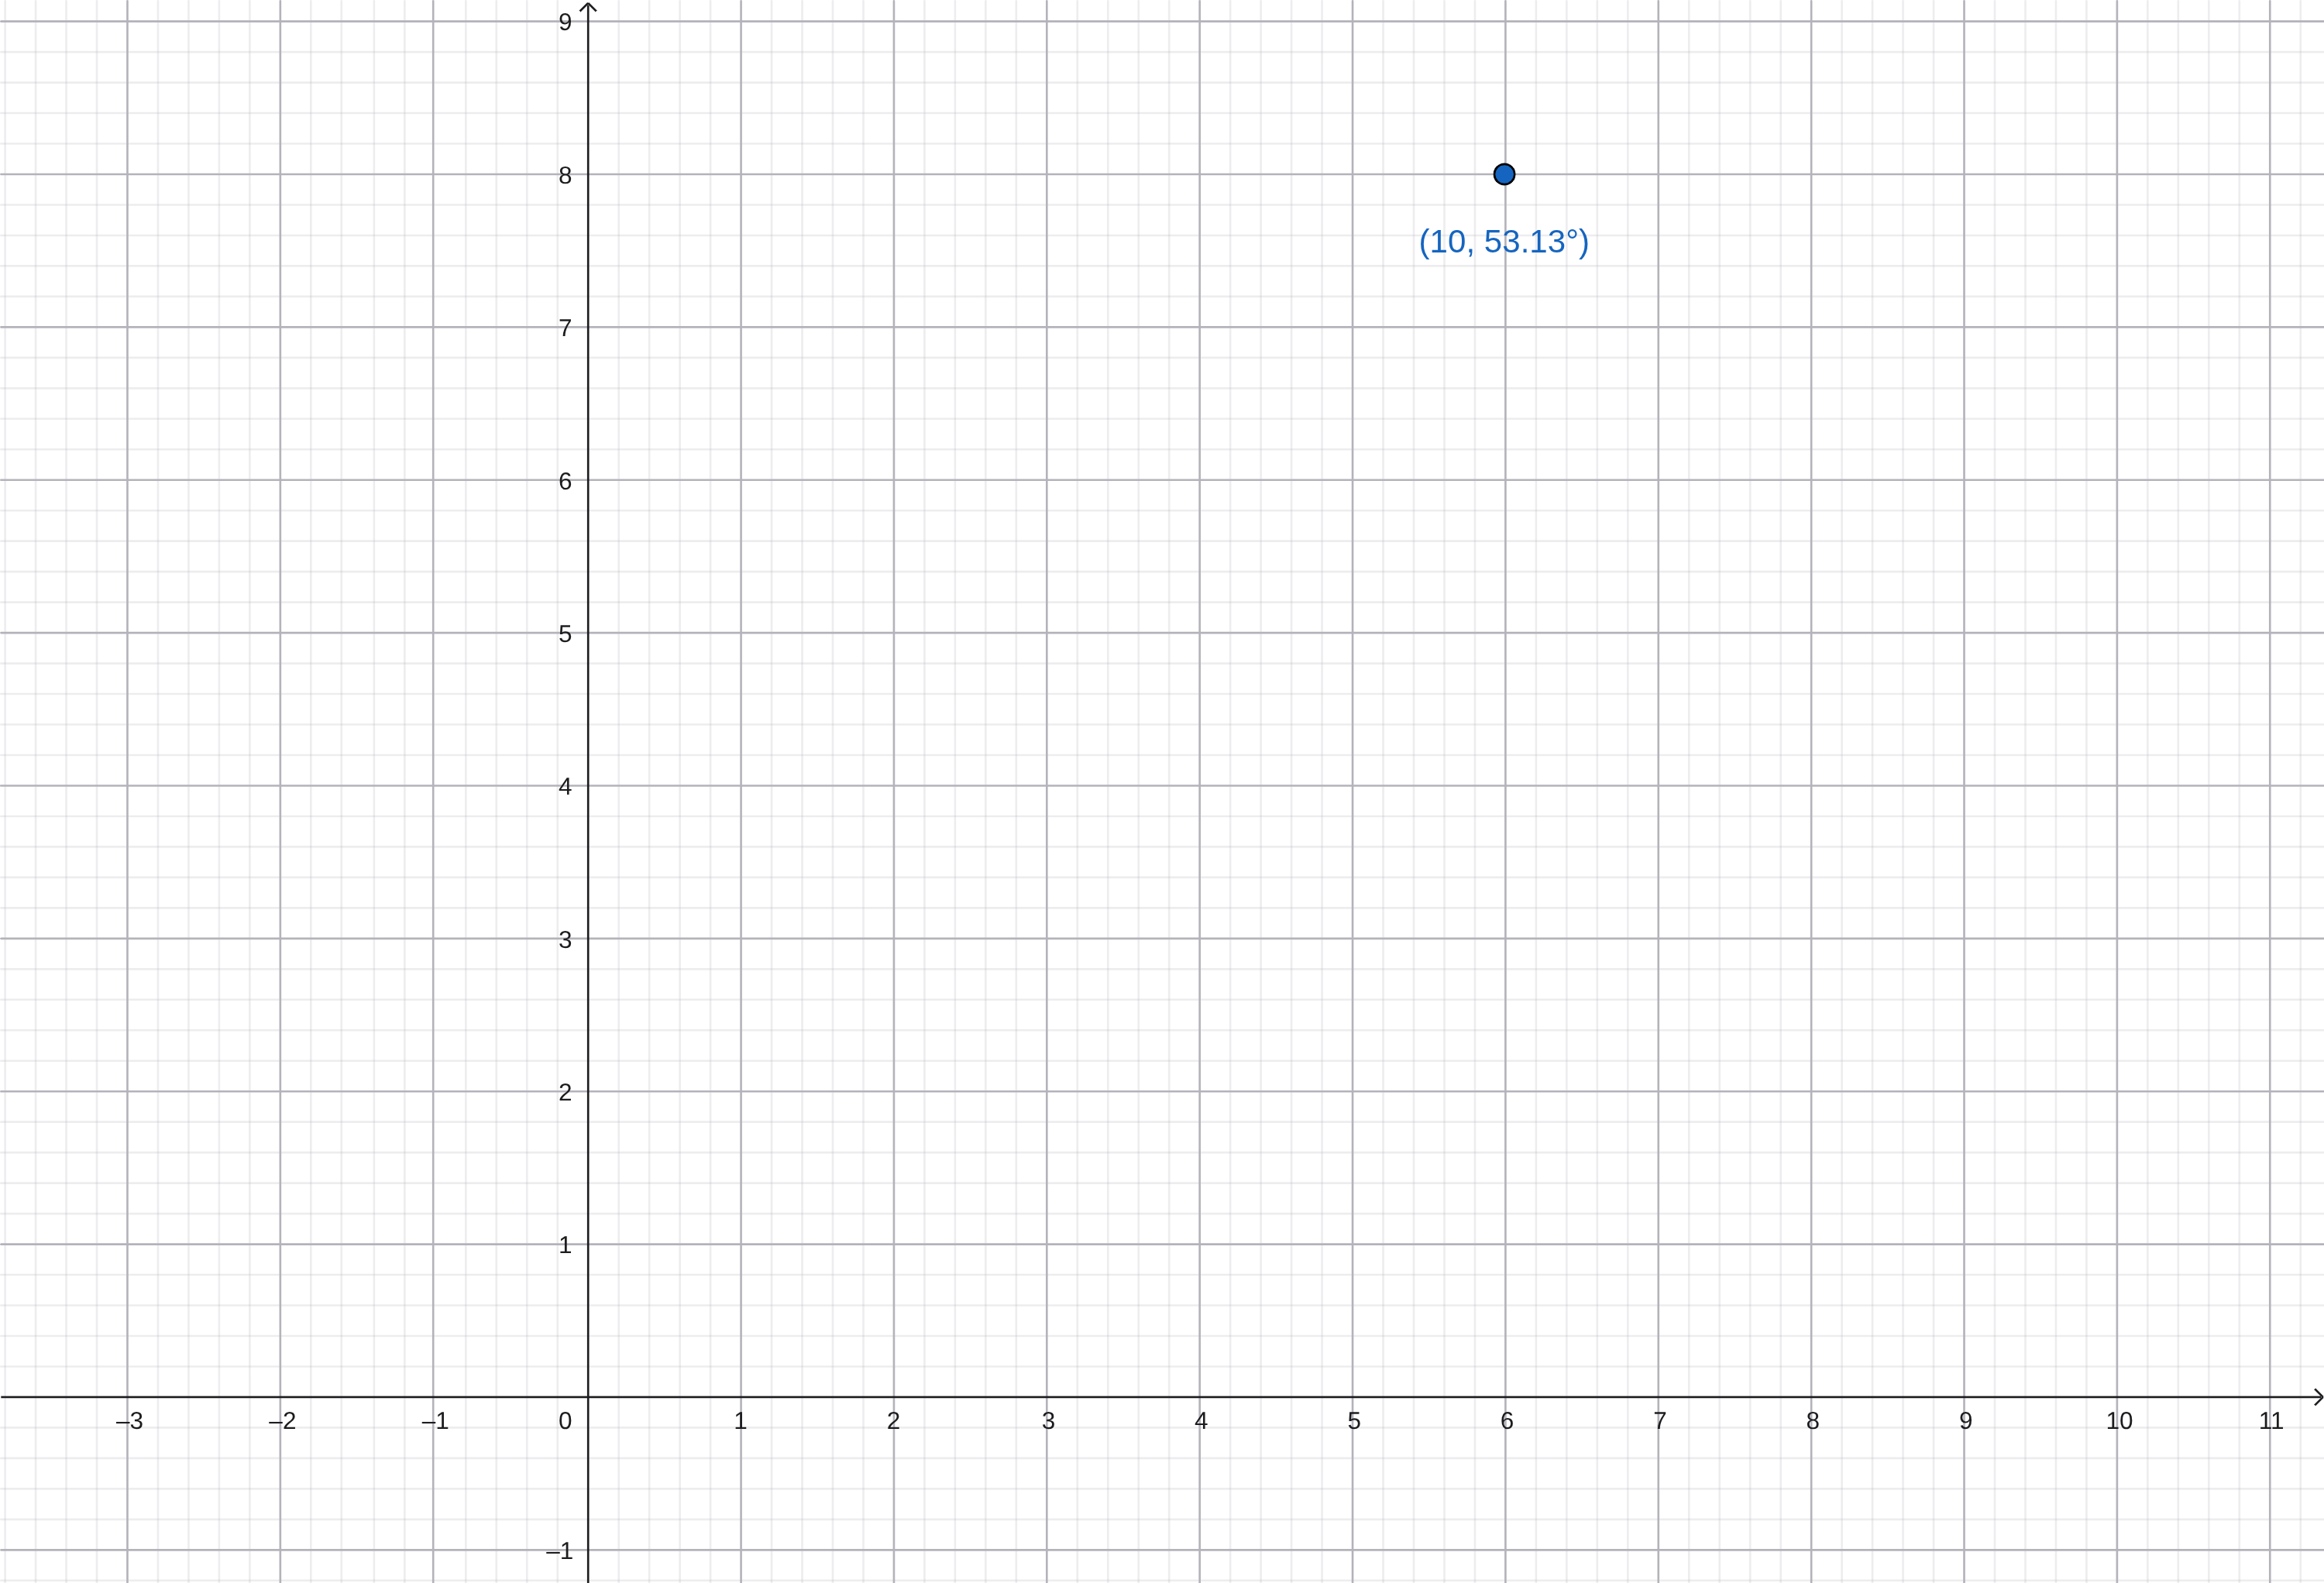
\includegraphics[width=0.4\linewidth]{./geogebra-export4.png}
	\caption{Ubicación de $(10, 53.13^\circ)$}
\end{figure}

% Actividad 3
\section*{Actividad 3}
\textbf{Instrucciones:} Una herramienta robótica gira $30^\circ$ y se extiende 20 $cm$. Determinar su posición cartesiana.
\newline

\textbf{Respuesta:}
\begin{align*}
	r &= 20 \\ 
	\theta &= 30^\circ \\
	\left(r, \theta\right) &\Longrightarrow (20, 30^\circ) \\
	\left(r, \theta\right) &\Longrightarrow \left(x, y\right) \\
	r &= \sqrt{x^2 + y^2} \\
	\theta &= \tan^{-1}\left(\frac{y}{x}\right) \\
\end{align*}

\begin{align*}
	\sin\theta = \frac{y}{r} &\Longrightarrow r\cdot\sin\theta = y \\
	&\Longrightarrow y = r\sin\theta \\
	\cos\theta = \frac{x}{r} &\Longrightarrow r\cdot\cos\theta = x \\
	&\Longrightarrow x = r\cos\theta \\
\end{align*}
\begin{align*}
	(x, y) &\Longrightarrow (r\cos\theta, r\sin\theta) \\
	&\Longrightarrow \left(20\cos30^\circ, 20\sin30^\circ\right) \\
\end{align*}

\begin{figure}[htb]
	\centering
	\begin{subfigure}[b]{0.40\linewidth}
		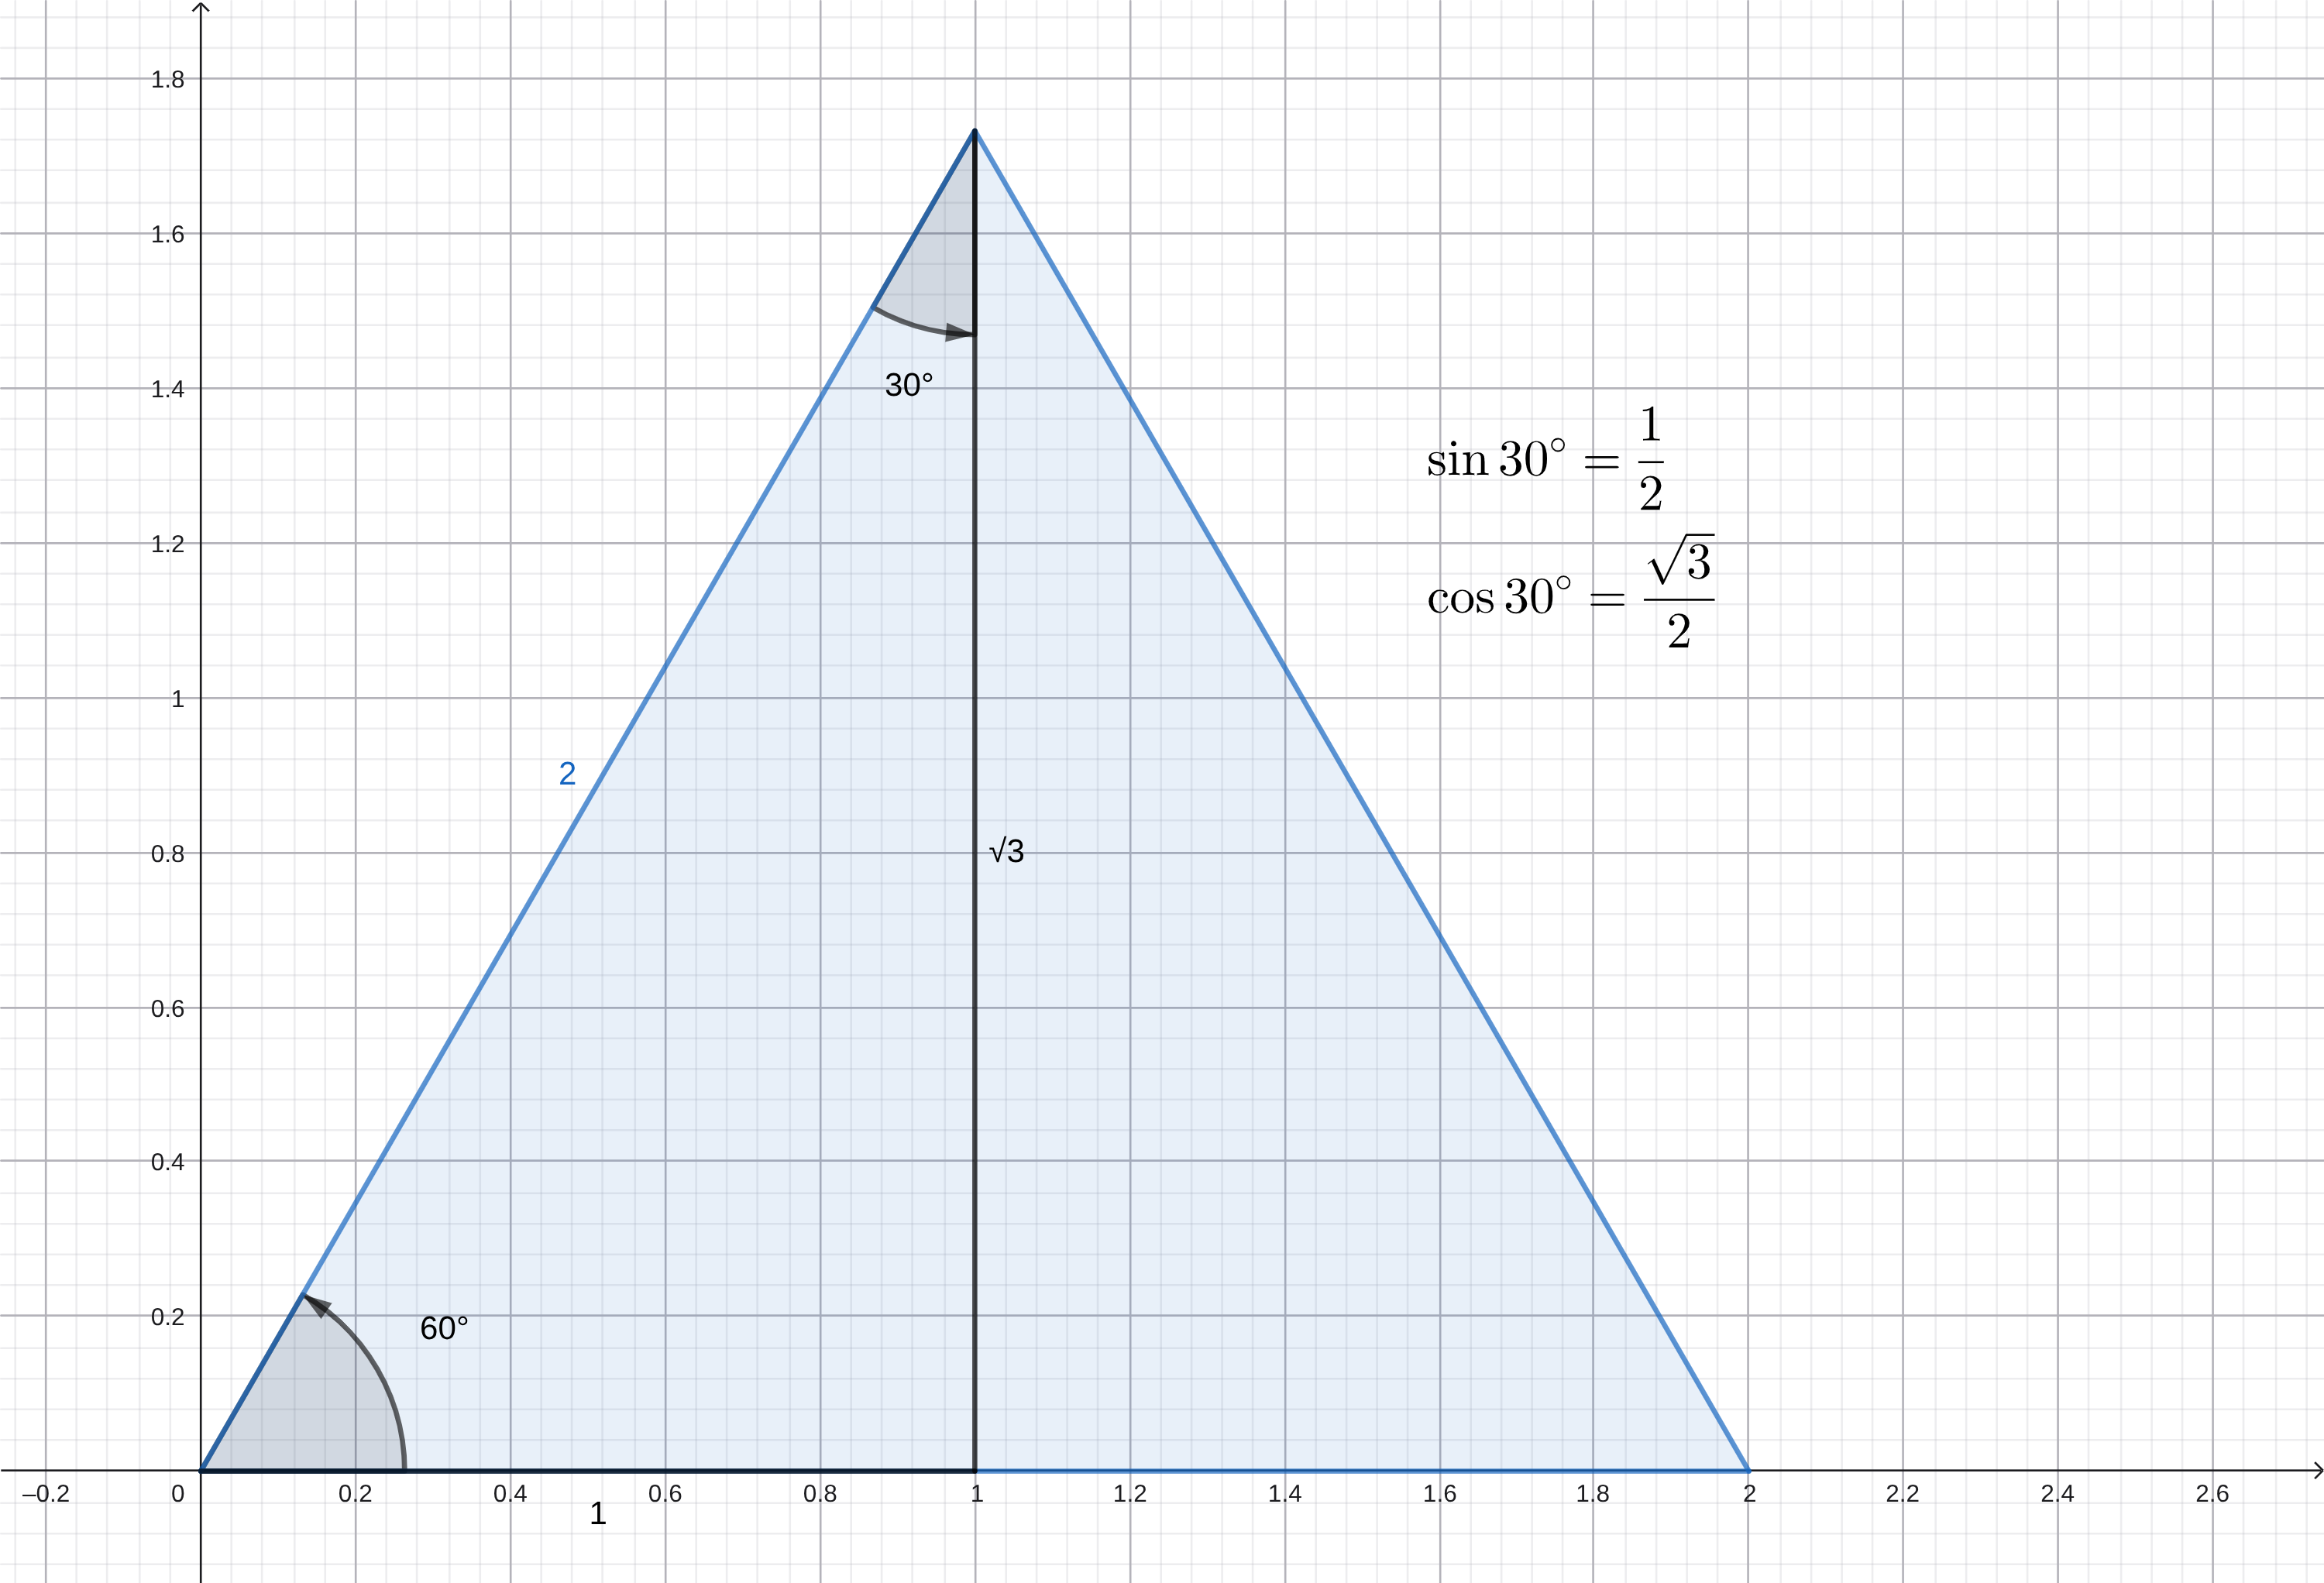
\includegraphics[width=\linewidth]{./geogebra-export2.png}
		\caption{$\sin$ y $\cos$ de $30^\circ$}
	\end{subfigure}
	\begin{subfigure}[b]{0.40\linewidth}
		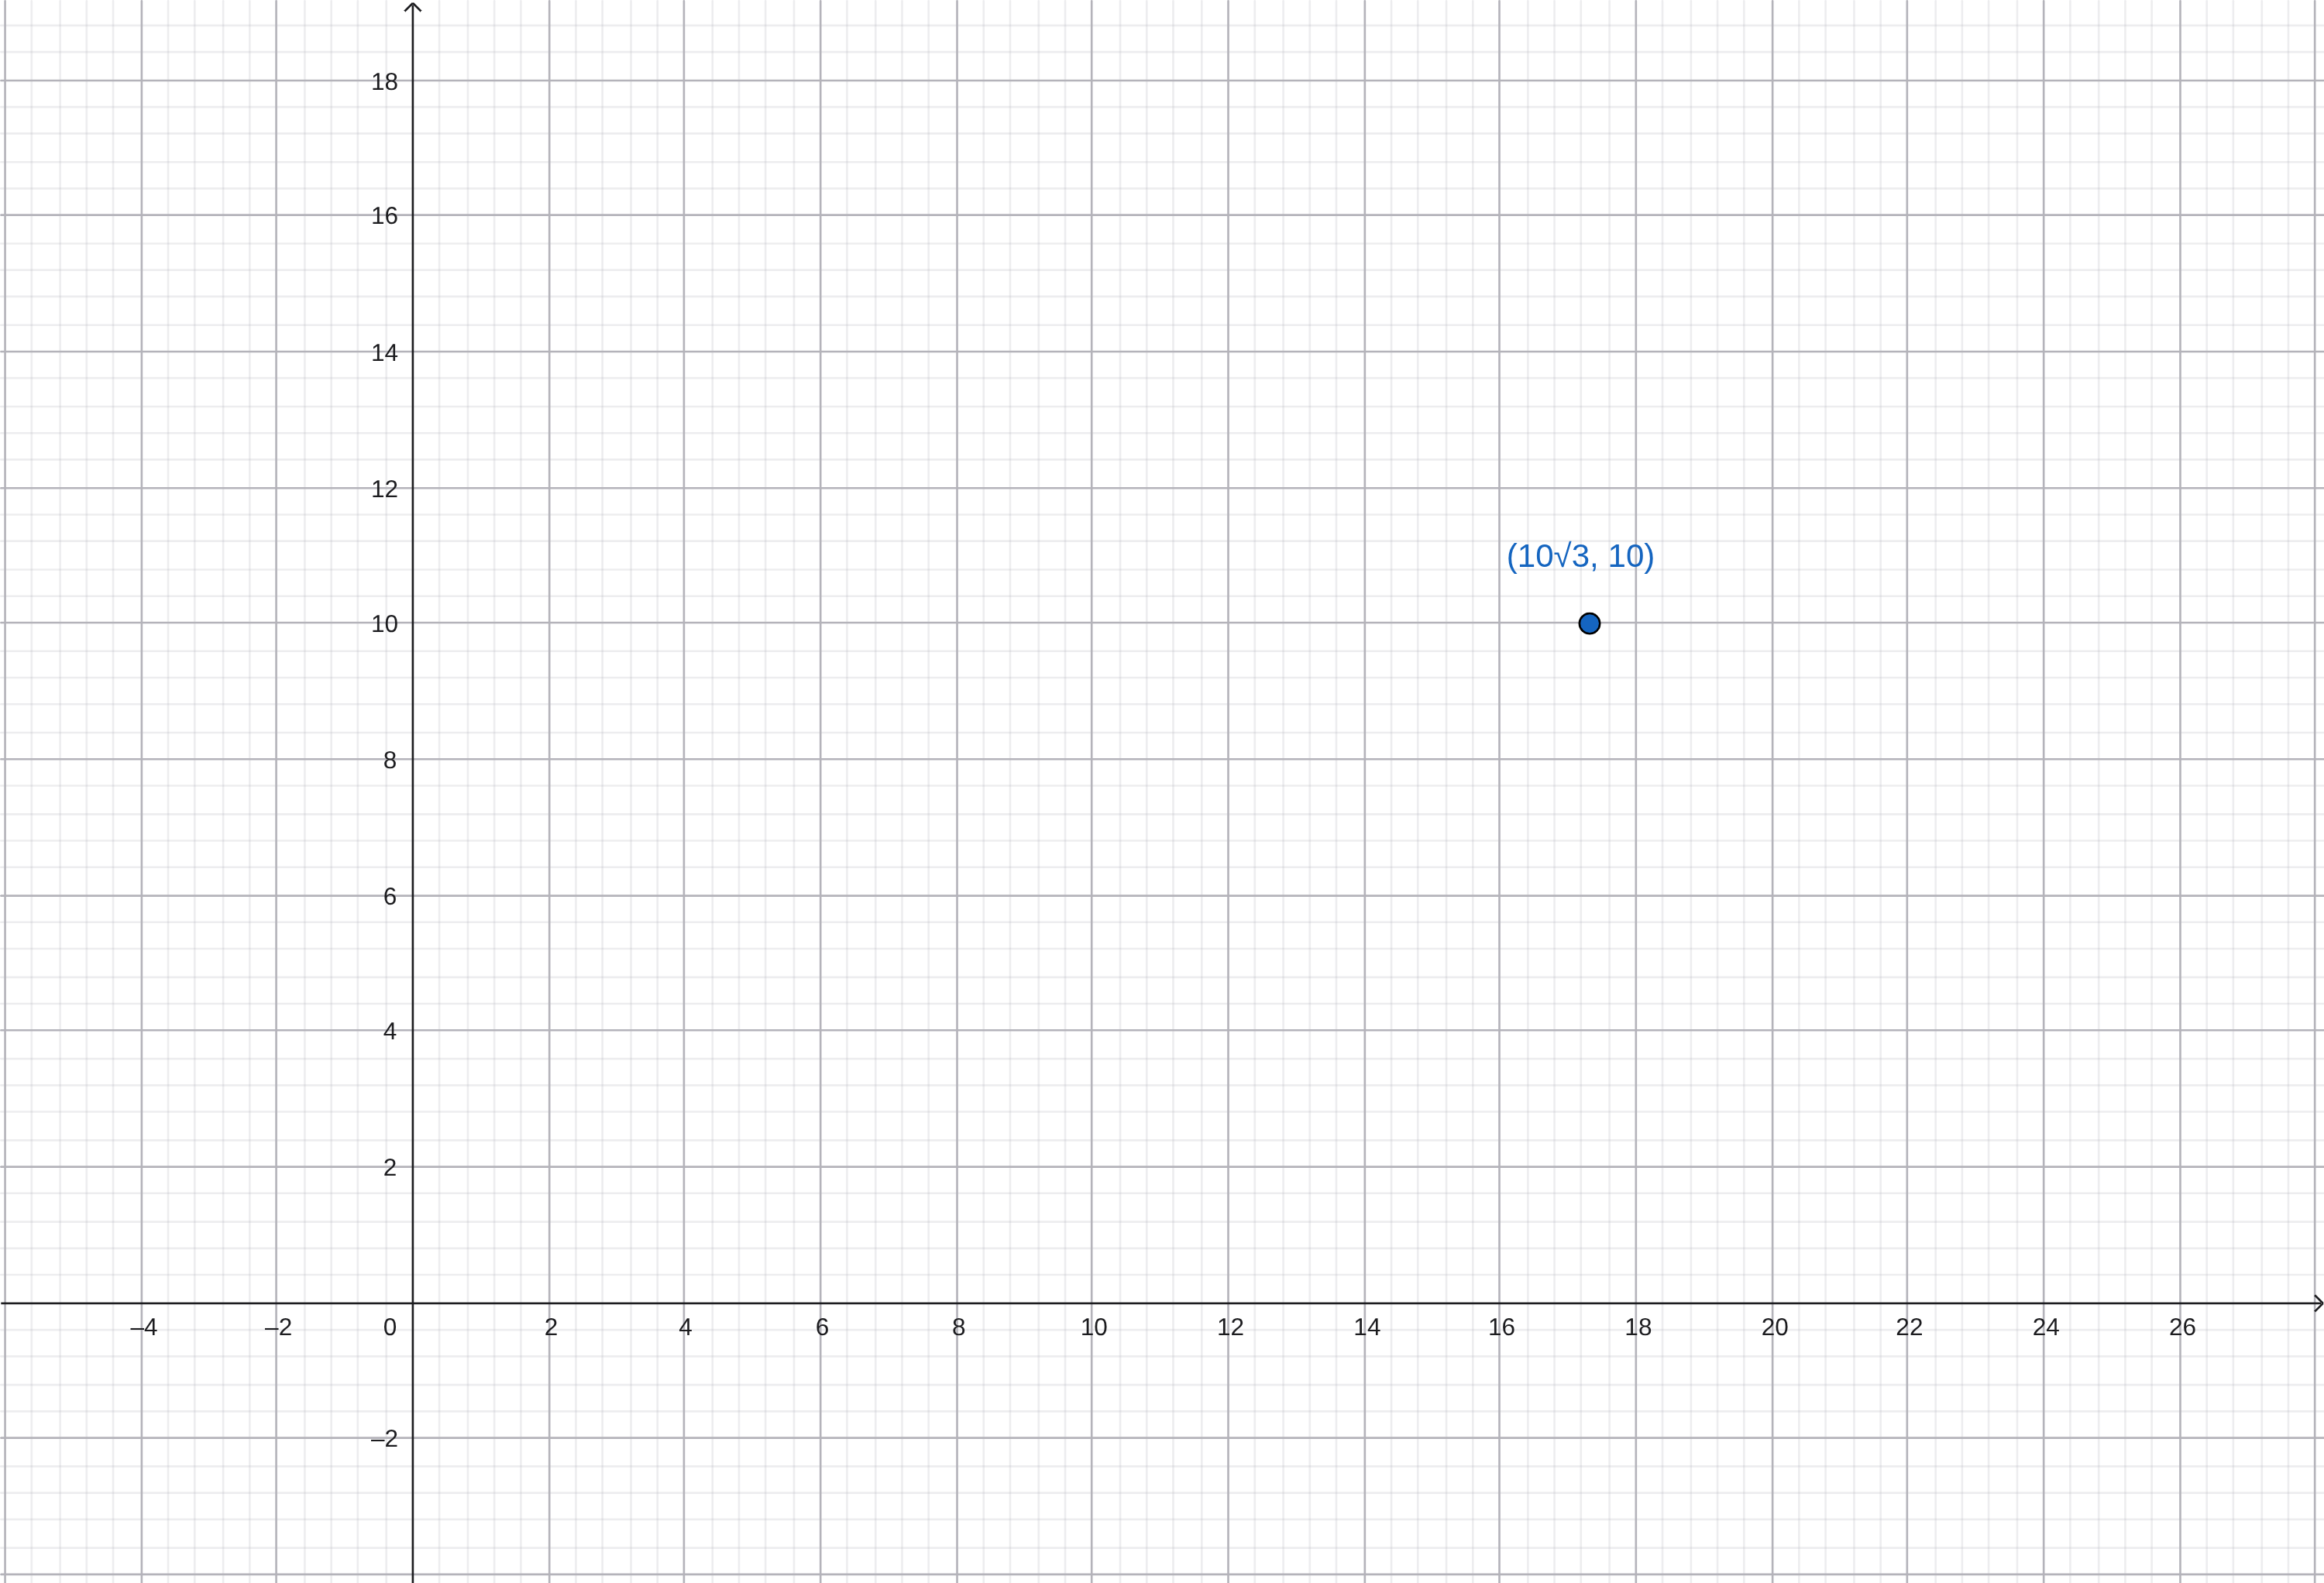
\includegraphics[width=\linewidth]{./geogebra-export5.png}
		\caption{Ubicación de $(10\sqrt{3}, 10)$}
	\end{subfigure}
\end{figure}

\begin{align*}
	\left(r\cos\theta, r\sin\theta\right) &\Longrightarrow \left(20\left(\frac{\sqrt{3}}{2}\right), 20\left(\frac{1}{2}\right)\right) \\
	&\Longrightarrow (10\sqrt{3}, 10) \\
\end{align*}
\end{document}
